\subsection{Interface}

As interfaces fornecem uma maneira de definir contratos entre diferentes
classes, portanto, uma interface pode definir: a assinatura de métodos e
valores armazenados através de constantes. Por conta disto, qualquer classe  que
quiser seguir os padrões definidos pela interface deverá assinar um contrato,
ou seja, deverá implementar a assinatura dos métodos da mesma maneira como  fora
definido na interface \cite{programmingPhp}.

Além disto permite abstrair recursos em sistemas e facilitar a
injeção de dependências, além de garantir a extensibilidade e padronização do
projeto, ou seja, é possível definir que um objeto irá receber como argumento de
um método construtor uma interface, sendo que, é permitido passar como parâmetro
qualquer classe que implemente a interface.

Agora será apresentado um exemplo referente a definição de uma interface
utilizando a linguagem PHP.







Por conta de um método, é possível que um objeto possa realizar chamadas 
permite que de fora da classe carro outro objeto configure a cor de um veículo passando uma mensagem ao objeto carro com a cor solicitada. Podemos ver
um exemplo desta situação na imagem abaixo:


Isto permite que fora da classe carro outro objeto configure a cor de um
veículo, na Figura \ref{fig:chamadaMetodo} é exibido um exemplo desta
situação:


\begin{figure}[h!tb]
	\caption{Chamada de um Método utilizando a linguagem PHP}
	\label{fig:chamadaMetodo}

	\centering
	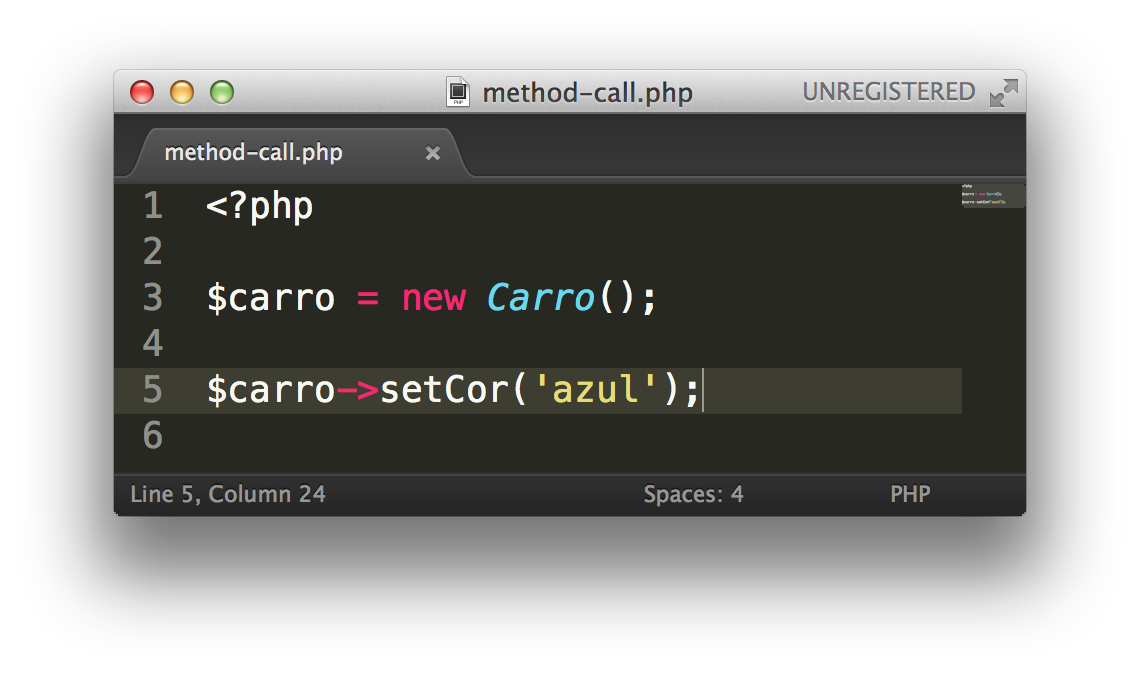
\includegraphics[width=0.6\textwidth]{images/method-call.png}

	\centering
	\footnotesize Fonte: \fonteOAutor
\end{figure}

\FloatBarrier 	% Este comando impede que as imagens
				% flutuem a partir deste ponto no seu documento

Abaixo, você irá conferir uma explicação referente ao código que foi
apresentado na Figura \ref{fig:chamadaMetodo}:

\begin{enumerate}[a)]
    \item linha 1: tem-se o início da execução de um bloco de código
    PHP;
    \item linha 2: ocorre a criação de um objeto do tipo \textit{Carro};
    \item linha 5: realiza-se a chamada de um método chamado
    \textit{setCor}, sendo que, informa-se um parâmetro para ele, que na
    linguagem \acs{PHP} representa uma \textit{string} (cadeira de caracteres). Logo,
    configura-se o valor da propriedade \textit{cor} da classe \textit{Carro}
    para receber o valor \textit{azul}.
\end{enumerate}